\subsection{\ac{SDS} build and integration}\label{SDS_build_and_integration}
The last step to complete the user story of the \ac{SDS} is to integrate the system into an application. This chapter explains how to package the \ac{SDS} and load it into the desired application. The integration must be simple, so it is not discouraging for developers using the design system.  \\

The build process is the first important part of understanding the integration workflow. Webpack is the build tool used by \ac{SDS}. As shown in Figure \ref{building_block_level_2_component_sds} in Chapter \ref{architecture_componens}, the design system's components use Typescript, including the Lit framework and using \ac{SCSS} for styling. Since the browser does not support Typescript and \ac{SCSS}, they must be processed beforehand. \\
Webpack uses a configuration file, often called \texttt{webpack.config.js}, to describe the steps in which steps Webpack compiles the code This file describes rules that tell Webpack what to do with which files come into the build pipeline. For example, these rules for \ac{SDS} look like this: \\
\lstinputlisting[linerange={23-41},firstnumber=23,caption={\ac{SDS} Webpack rules},label=WebpackRules]{../Code/webpack.config.js}
TThe rules define regular expressions assigning files with extensions to the corresponding compilers. In the Webpack world, their name is loaders. The loaders used here are build-in. However, the build process also integrates custom ones. When using loaders, it is sufficient to include the loader string in the \texttt{use} property of a rule object. For example, in lines 25-26, Listing \ref{WebpackRules}, the Typescript loader is matched with the regular expression Typescript to process Typescript files. The same pattern in lines 34-35, Listing \ref{WebpackRules}, matches \ac{SCSS} files with the default style loader within Webpack. \\
After all declarations of rules for compilation, it is time to define the entry point from which Webpack should start building the project. The \texttt{entry} property in the \texttt{webpack.config.js} file defines the starting point. In the case of \ac{SDS}, the starting point is \texttt{./src/index.ts}. Since there is only one entry point, this file is responsible for all files needed for \ac{SDS}. For example, looking at the entry file in Listing \ref{IndexSDS} shows that there are several imports of Typescript and styling files. 
\lstinputlisting[linerange={1-9},firstnumber=1,caption={\ac{SDS} Webpack rules},label=IndexSDS]{../Code/src/index.ts}
The first six lines of the \texttt{index.ts} contain the imports of all components written in the \ac{SDS} so far. A defined alias in the \texttt{tsconfig.json} and \texttt{webpack.config.js} allows shortening the import path for components. With the import of the component files, which look similar to the button component presented above, the browser automatically adds the web components as custom elements and are ready for use in the browser. In the future, this import might change, as software might not want to load all components at once. \\
The last three lines from 7-9 represent imports of styles. Again, a single large file could hold all these styles, but the design system splits them for readability. These files contain defined design tokens for colors, spacing and sizes for components, and patterns. As an example, the \texttt{colors.scss} looks like this:
\lstinputlisting[linerange={1-15},firstnumber=1,caption={\ac{SDS} color design tokens},label=ColorTokens]{../Code/src/atoms/colors.scss}
The styling file consists mainly of defined \ac{CSS} variables. Any software that loads the design system can overwrite these. By changing these rules, all components in the entire design system receive style changes. A documentation page provides all information (Figure \ref{sds_color_design_tokens}), so it is not necessarily going into the design system code to find them.
\begin{figure}[htbp]
    \centerline{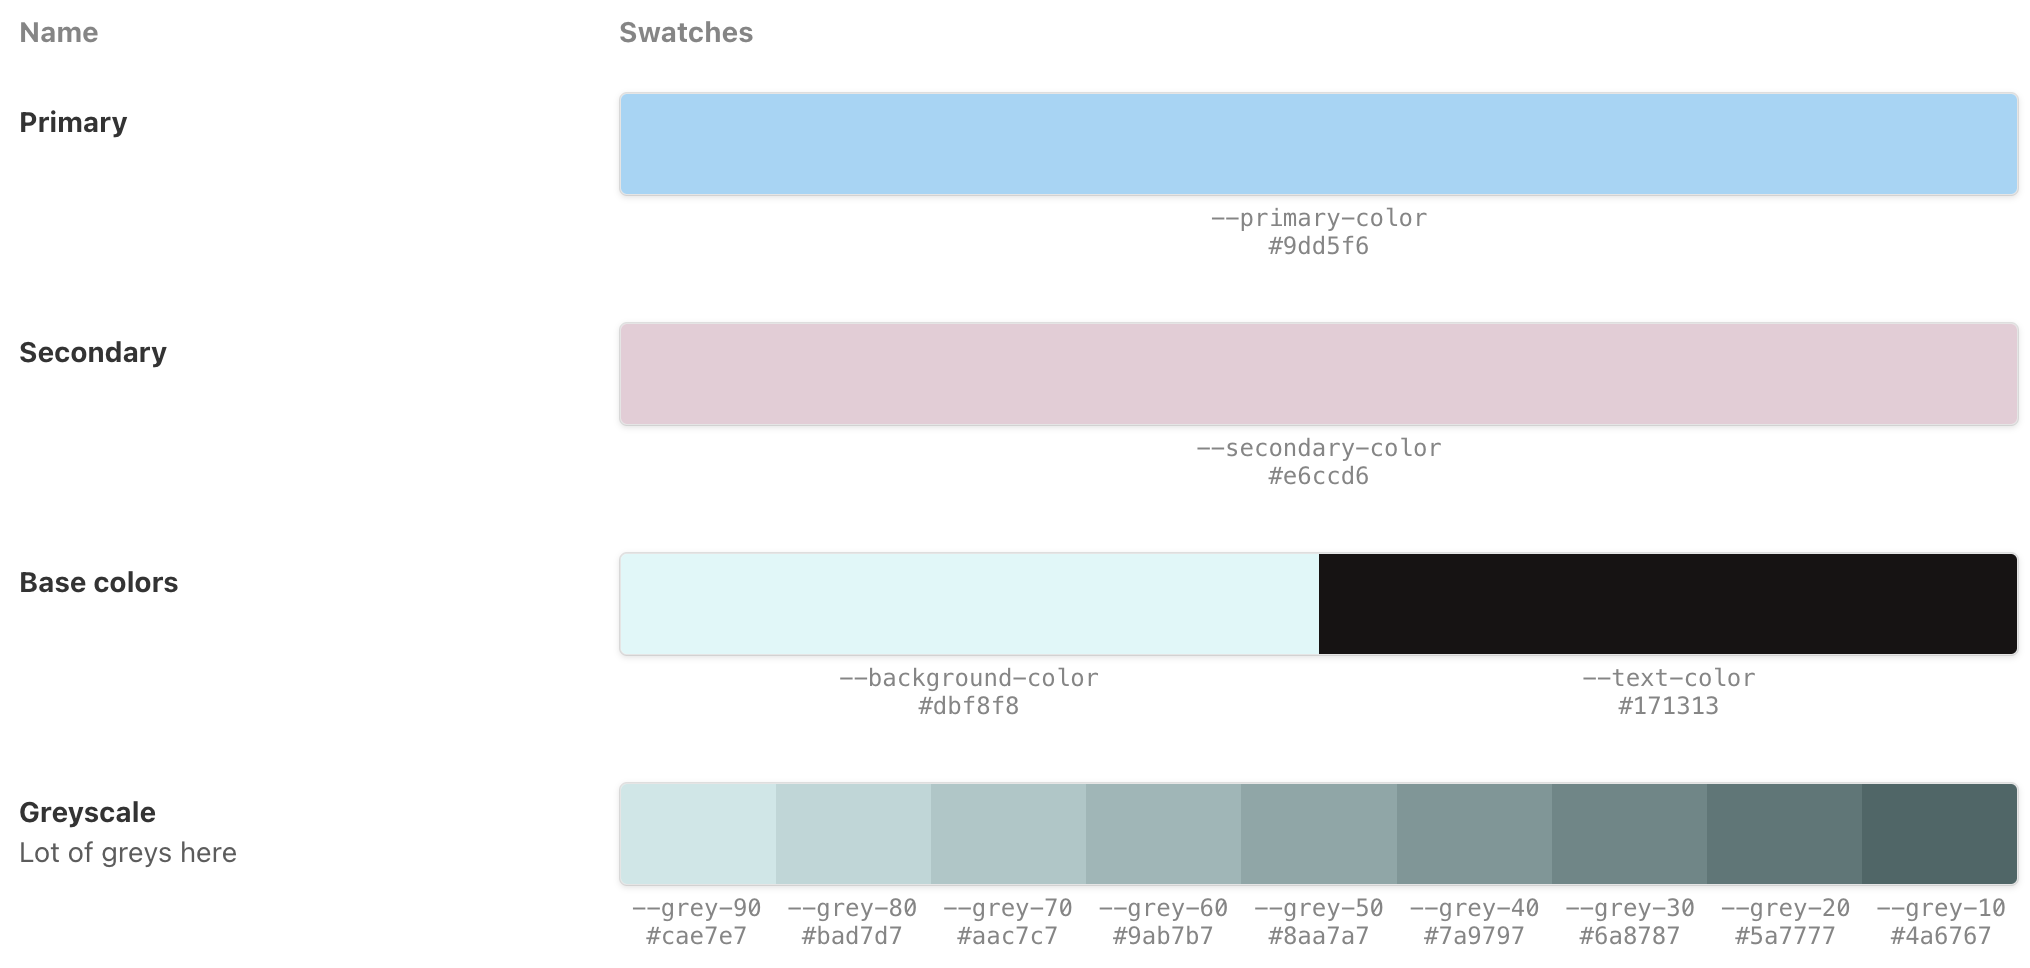
\includegraphics[width=\linewidth]{images/color_design_tokens.png}}
    \caption{\ac{SDS} color design tokens documentation}
    \label{sds_color_design_tokens}
\end{figure} \\
At a later stage in the design system, the complexity of the styling files may change. For this reason, the \ac{SDS} uses \ac{SCSS} to take advantage of its feature of using mixins to create more complex rule sets.\citep{scss_sass_nodate} \\
After the compiler transforms all source files into browser-readable code, it bundles the sources into two files. One file contains the Javascript code. This code registers the custom elements and provides the logic needed in them. The other file, due to the build process, is a \ac{CSS} file containing all the styles defined in the previously included design token files. For the design system to work correctly, applications must include both files. \\

Last but not least, projects load the bundled files. The design system uses a so-called package manager such as \acl{NPM} to make components and tokens globally available to all.In the case of this elaboration, it omits the step to publish the bundled files. Instead, the application loads the files directly from the build folder into the project. The files can either be loaded via \texttt{<script>} and \texttt{<link>} tag within an \ac{HTML} file or included in the project's build process. The only requirement is that they are both included. \\
In conclusion, this chapter presents an overview of the \ac{SDS} build and integration into existing or new projects. The next chapter will look at a project that uses \ac{SDS} and compare it to a project that does not. Finally, testing both software will shed light on whether such a design system can contribute to the standardization of user interfaces for \ac{SaaS} software. 